%!TEX root = ../../main.tex
\section{Incorporating the RDE into DWD Calculations}
\label{sec:Incorporating the RDE into DWD Calculations}
The RDE is a monotonically decreasing function of the dose which is bounded between the values of 0 and 1 (equation \ref{eqrdeleal}).
If $\eta = \text{RDE}$ then the decreasing nature of the RDE means that as the dose increases, the DWD defined in equation \ref{eq:DWD equation with RDE} will decrease at some point.
This may be a desirable characteristic if only diffraction is to be considered.
However if the DWD is used to characterise the damage in a crystal, then it would be expected to always increase with increasing radiation exposure.
For this reason two forms of $\eta$ were investigated along with the simple DWD where $\eta$ had no dose dependence:
\begin{align}
    \eta &= 1 \qquad \text{simple $\eta$ form}, \label{eq:Simple eta form} \\
    \eta &= \text{RDE} \qquad \text{deacreasing $\eta$ form}, \label{eq:Decreasing eta form} \\
    \eta &= 1 - \text{RDE} \qquad \text{increasing $\eta$ form} \label{eq:Increasing eta form}
\end{align}
Both dose dependent forms are bounded between 0 and 1.
The difference between them is that equation \ref{eq:Decreasing eta form} decreases from 1 to 0 whereas equation \ref{eq:Increasing eta form} increases from 0 to 1 as shown in Figures~\ref{fig:Decreasing Eta} and \ref{fig:Increasing Eta} respectively.
\begin{figure}
        \centering
        \begin{subfigure}[b]{0.45\textwidth}
                \centering
                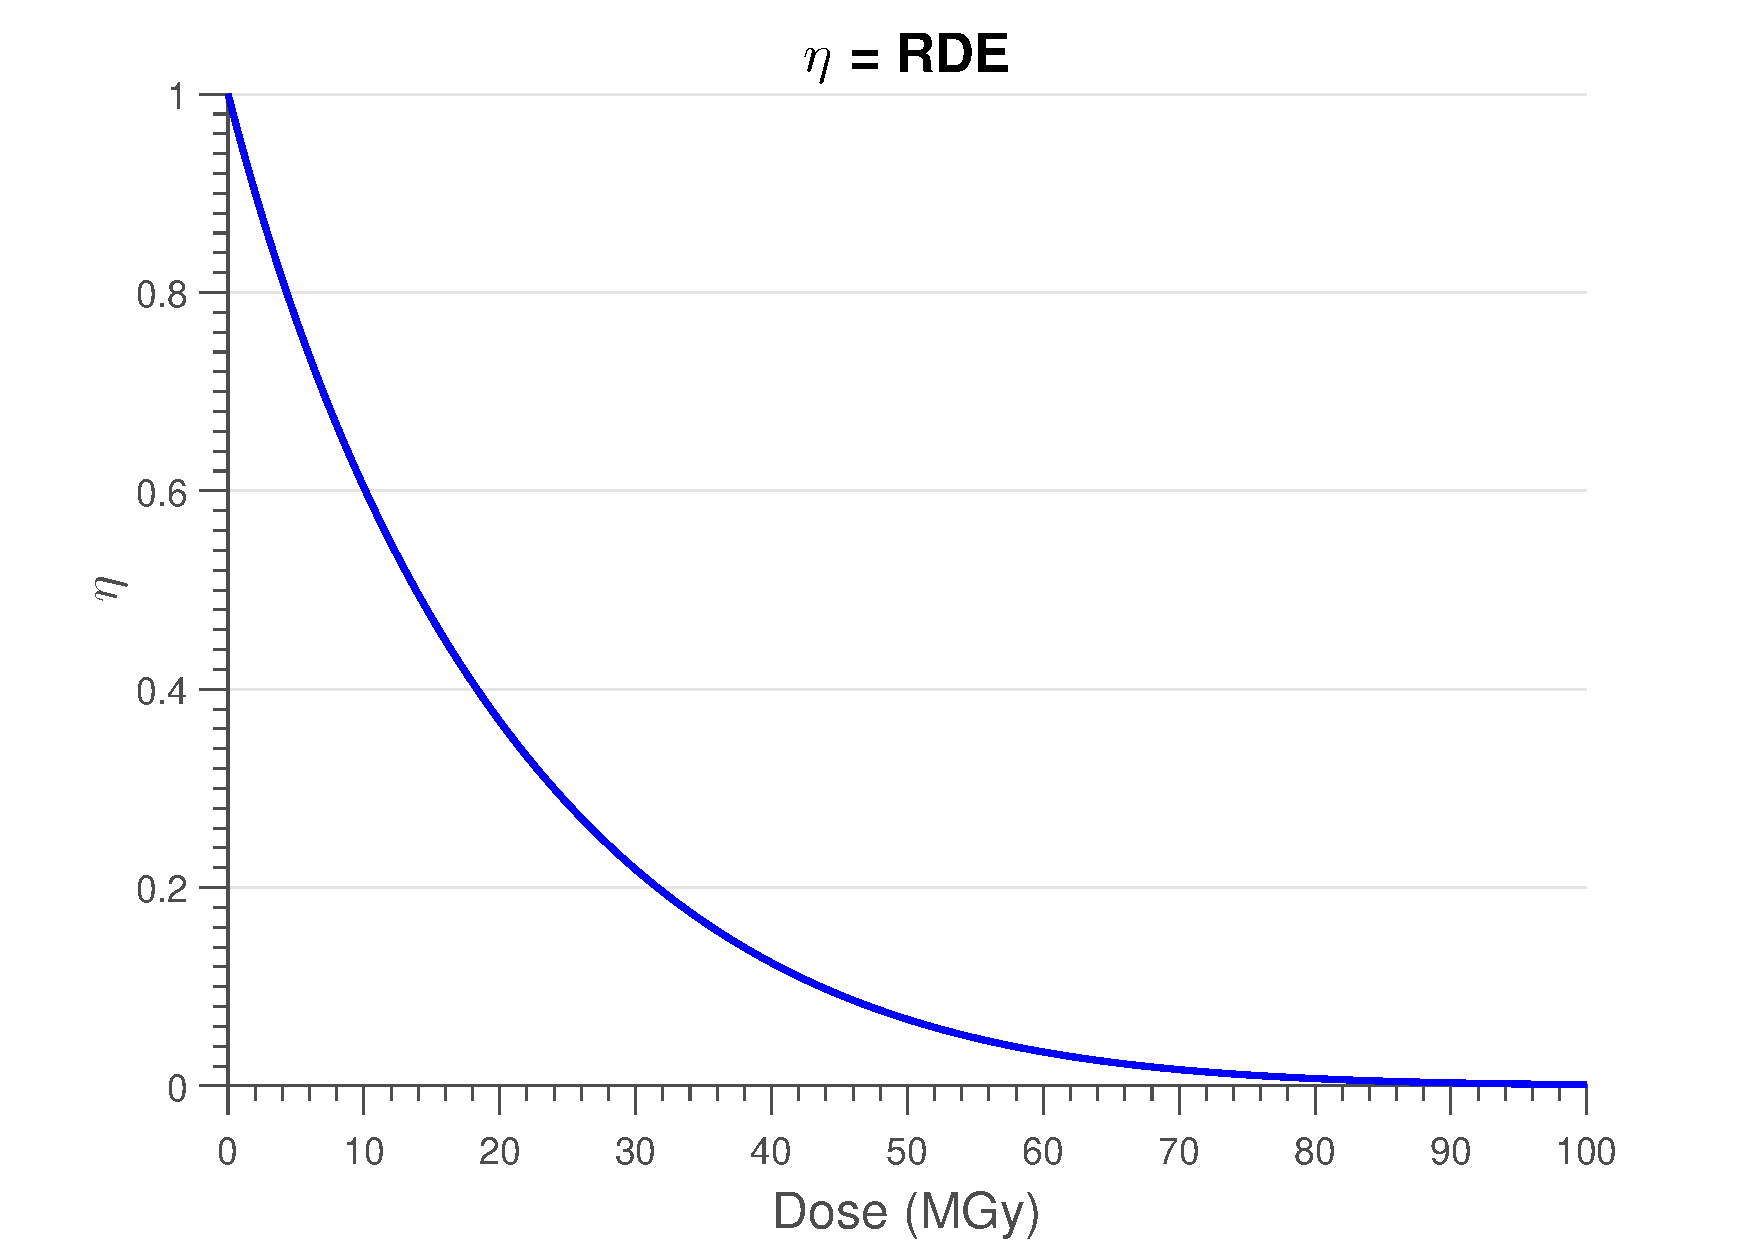
\includegraphics[width=\textwidth]{figures/dwd/EtaDecreasing.pdf}
                \caption{}
                \label{fig:Decreasing Eta}
        \end{subfigure}
			\quad
        \begin{subfigure}[b]{0.45\textwidth}
                \centering
                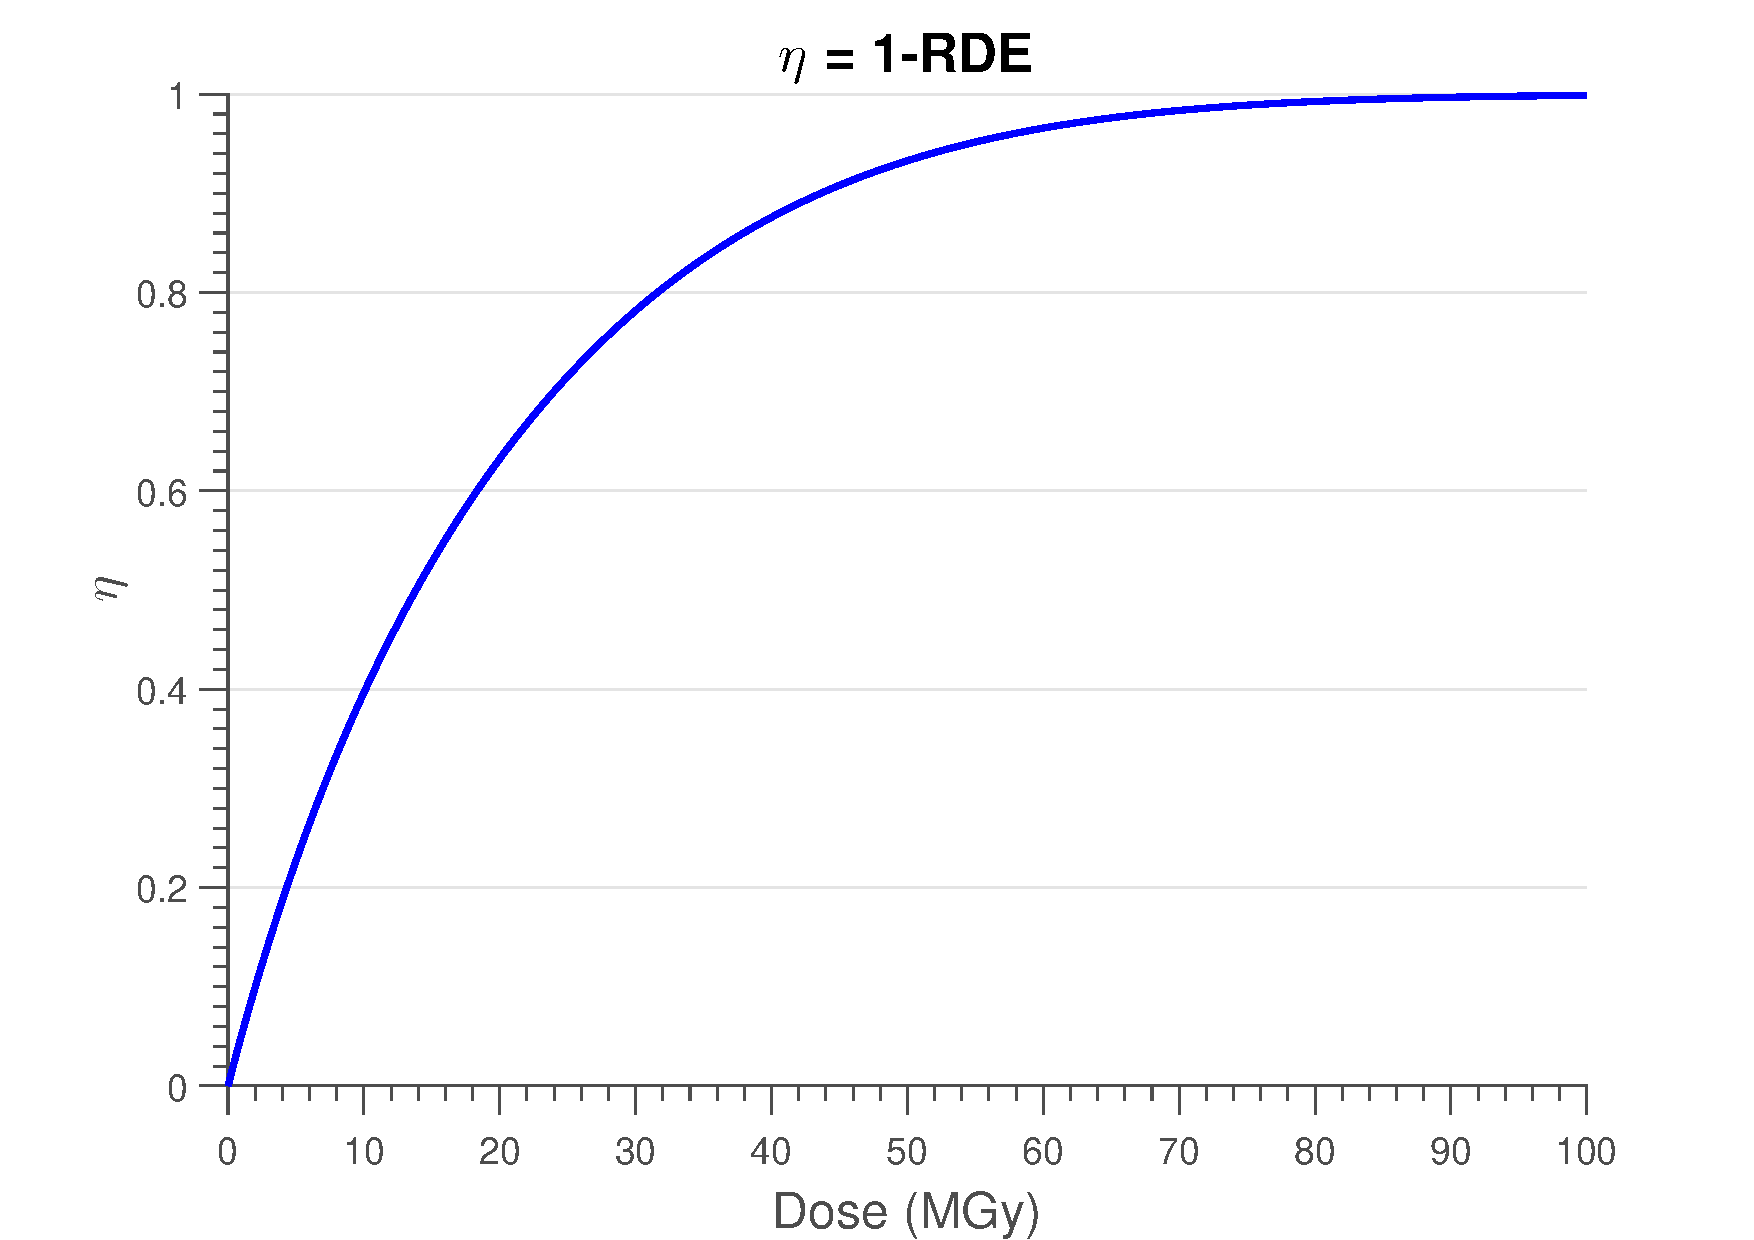
\includegraphics[width=\textwidth]{figures/dwd/EtaIncreasing.pdf}
                \caption{}
                \label{fig:Increasing Eta}
        \end{subfigure}
        \caption{Two different forms of $\eta$ used in equation \ref{eq:DWD equation with RDE}. (a) $\eta = \text{RDE}$. (b) $\eta = 1-\text{RDE}$.}
        \label{fig:Different Eta forms}
\end{figure}

The remainder of this section presents the results of the analysis carried out with the data from \cite{zeldin2013dwd} using the forms of $\eta$ given above, comparing their performance with the simple DWD (equation \ref{eq:DWD equation - no RDE}).

\subsection{Predicting intensity loss}
\label{sub:Predicting intensity loss}
In the study carried out by Zeldin \textit{et al.} \cite{zeldin2013dwd} cubic crystals of bovine pancreatic insulin were irradiated under different dose contrast conditions.
The three beams used in the study: big, medium and small, can be seen in Figure~\ref{fig:Big, medium and small beams - Oli experiment}.
\begin{figure}
  \centering
    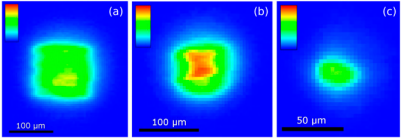
\includegraphics[width=1\textwidth]{figures/dwd/Oli_beams.png}
    \caption{False color images of the beam profiles used for the experiments in \cite{zeldin2013dwd}.
    The pixel size is $\text{5} \times \text{5}\,\mu m^2$ in all cases.
    (a) big beam, (b) medium beam and (c) Small beam.}
    \label{fig:Big, medium and small beams - Oli experiment}
\end{figure}
It was shown that the DWD is a significantly better metric for assessing the extent of radiation damage compared to the average dose for the whole crystal (AD-WC) or the maximum dose, because the spread of relative intensity values around the line of best fit of the data was greatly reduced (plots A-C in Figure~\ref{fig:Dose metric comparisons - zeldin et al} reproduced from \cite{zeldin2013dwd}).
The data for the big and small beams were available so the analysis performed by Zeldin \textit{et al.} in \cite{zeldin2013dwd} was repeated for each of the $\eta$ forms.
The results are shown in Figure~\ref{fig:Relative intensity - DWD eta forms}.
The main difference that can be seen from the plots is the DWD range.
The increasing $\eta$ function results in the largest range of DWD values.
Conversely, the decreasing $\eta$ function reduces the range of DWD values when compared to the simple DWD.
Another difference is that introducing a dose dependent $\eta$ function shifts the big beam data relative to the small beam data.
The increasing $\eta$ function shifts the big beam data towards higher dose values relative to the small beam data, whereas the decreasing $\eta$ function shifts the big beam data towards lower dose values.
This suggests that there is a signature from the different beams.
However this is an undesirable feature because DWD should already account for the different beam conditions via the flux weighting.
\begin{figure}
	\centering
    \begin{subfigure}[b]{1\textwidth}
        \centering
        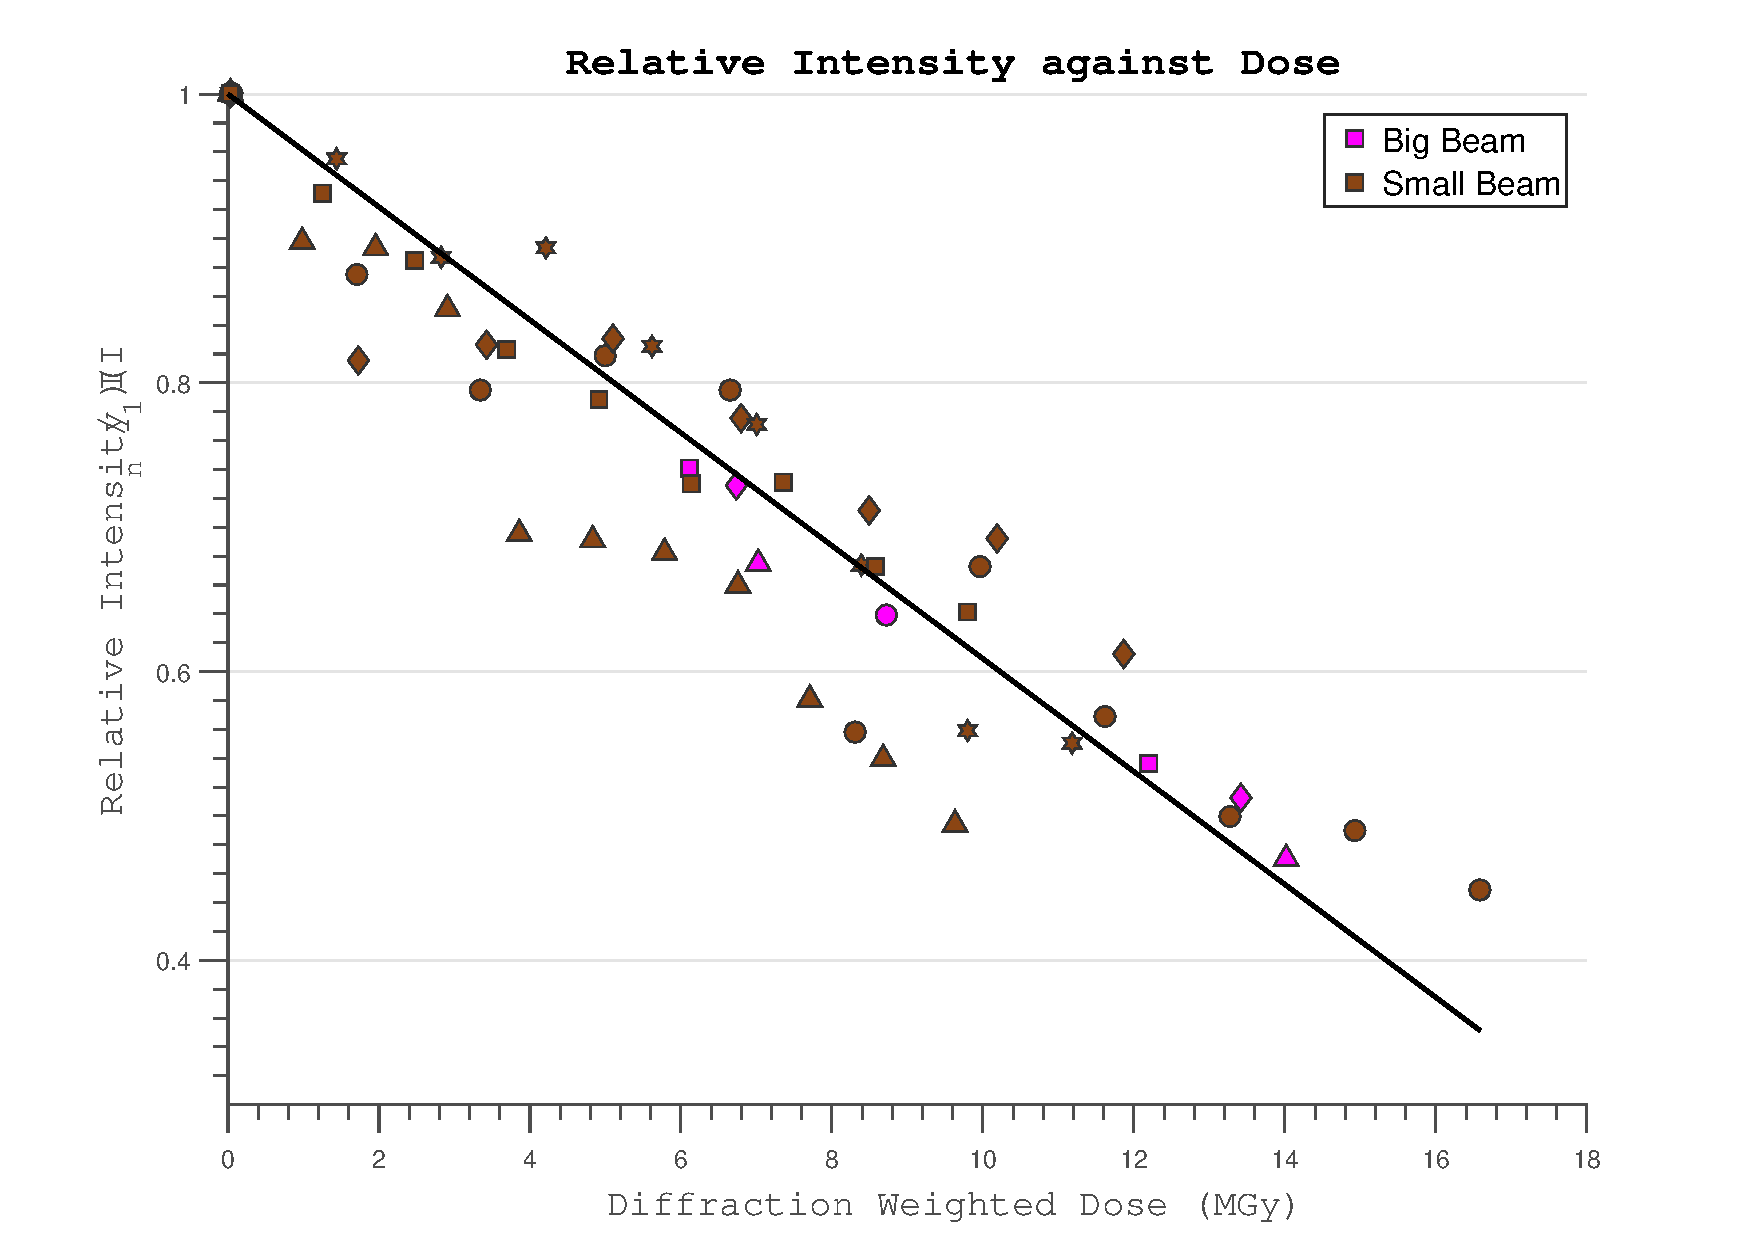
\includegraphics[width=\textwidth]{figures/dwd/reproduce_relint_DWDsimple.pdf}
        \caption{}
        \label{fig:Relative intensity - Simple DWD}
    \end{subfigure}
    \\
	\begin{subfigure}[b]{1\textwidth}
        \centering
        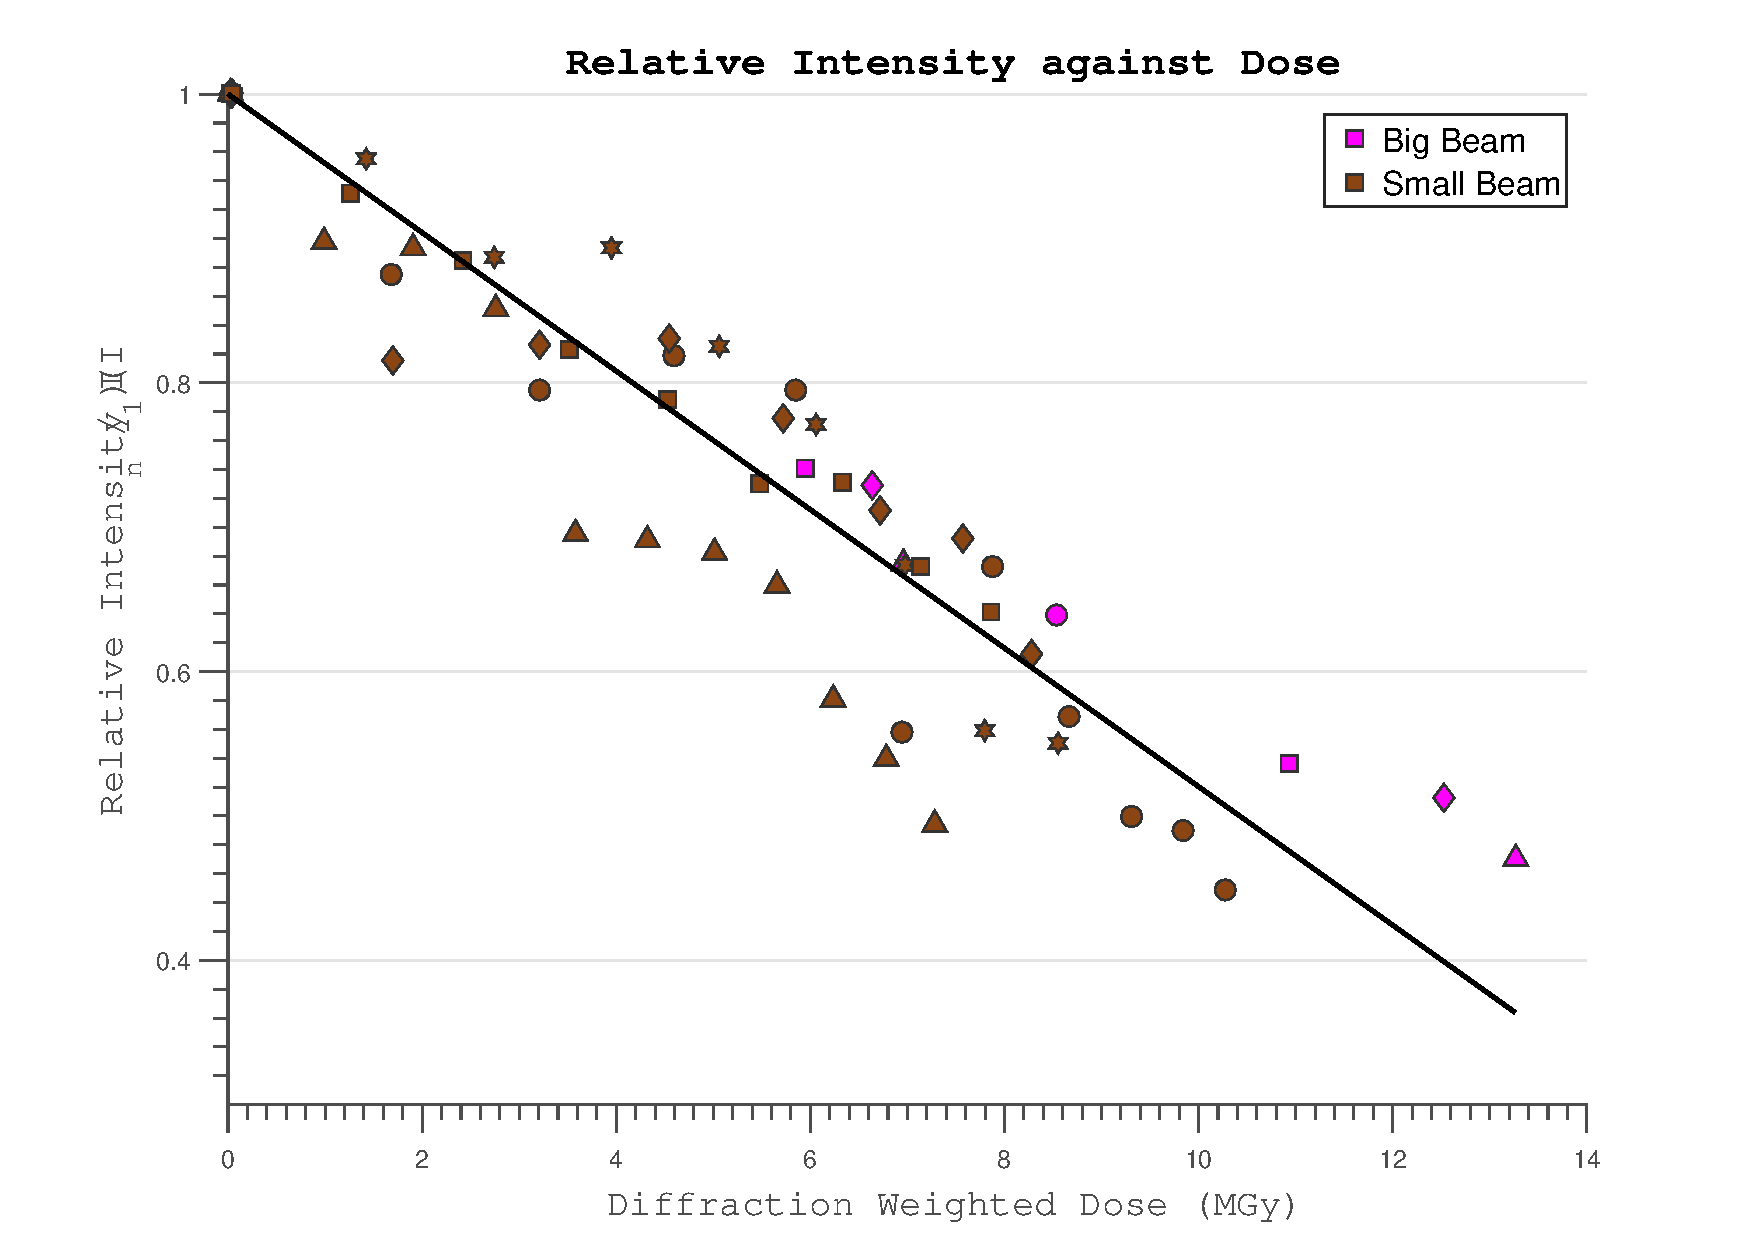
\includegraphics[width=\textwidth]{figures/dwd/reproduce_relint_DWDwrong.pdf}
        \caption{}
        \label{fig:Relative intensity - Increasing Eta}
    \end{subfigure}
\end{figure}
\begin{figure}
\ContinuedFloat
    \begin{subfigure}[b]{1\textwidth}
        \centering
        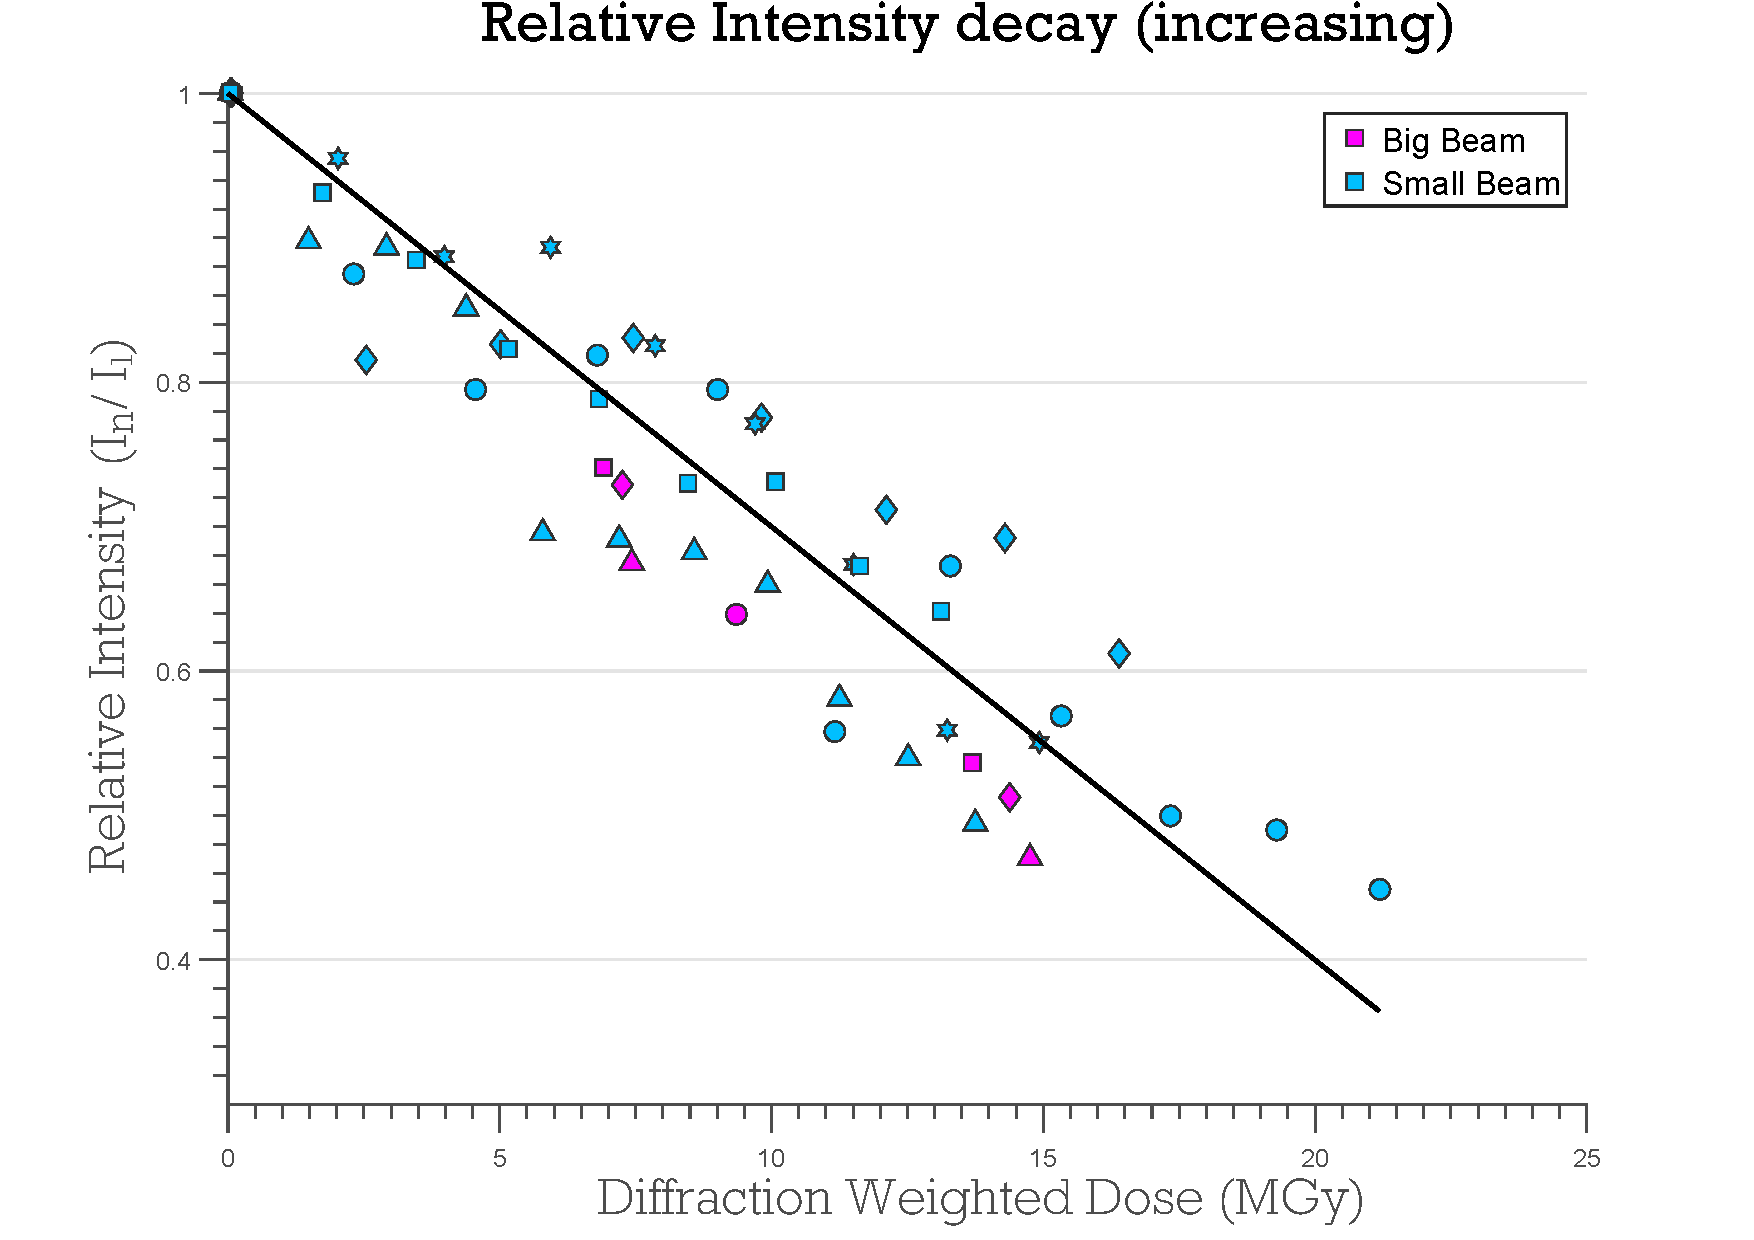
\includegraphics[width=\textwidth]{figures/dwd/reproduce_relint_DWDnew.pdf}
        \caption{}
        \label{fig:Relative intensity - Decreasing Eta}
    \end{subfigure}
	\caption{Relative intensity decay against the DWD using the different forms of $\eta$ given by equations \ref{eq:Simple eta form}, \ref{eq:Decreasing eta form} and \ref{eq:Increasing eta form}.
    (a) Simple $\eta$.
    (b) Decreasing $\eta$.
    (c) Increasing $\eta$.}
	\label{fig:Relative intensity - DWD eta forms}
\end{figure}

A line of best fit was calculated using a least squares fitting procedure and plotted (solid black line Figure~\ref{fig:Relative intensity - DWD eta forms}).
A measure of the overall deviation of the data from the line was obtained by calculating the squared Euclidean norm\footnote{The squared Euclidean norm is defined as $\sum_i (f(x_i) - y_i)^2$} for each DWD form (Table~\ref{tab:Squared Euclidean norm values - Relative intensity fits}).
The DWD form that gave the lowest value for the squared Euclidean norm was the simple DWD form.
This suggests that the data are less spread overall without adding a dose dependent form for $\eta$.
\begin{table}[ht!]
\small
\captionsetup{justification=centering}
	\caption{Squared Euclidean norm values of the line of best fit with the data in Figure~\ref{fig:Relative intensity - DWD eta forms}.}
	\centering
	\begin{tabular}{p{5cm} p{4.5cm}}
		$\eta$ form			                & Squared Euclidean norm    \\
		\hline
		$\eta = 1$ (simple)     			& 0.2034        \\
		$\eta = RDE$ (decreasing)     	    & 0.2112        \\
		$\eta = 1-RDE$ (increasing)    		& 0.2060       \\
		\hline
	\end{tabular}
	\label{tab:Squared Euclidean norm values - Relative intensity fits}
\end{table}

$D_{1/2}$ is a metric of the radiation sensitivity of a protein crystal that is defined as the dose at which the relative intensity falls to 50\%.
$D_{1/2}$ values were calculated from the line of best fit for each of the DWD forms.
Furthermore $s_{AD}$ values (as defined in section \ref{subs:Relative B factor}) were also calculated and both sets of values are given in Table~\ref{tab:Half dose and SAD values}.
\begin{table}[ht!]
\small
\captionsetup{justification=centering}
	\caption{Parameter values for Leal \emph{et al.} model determined by the method described in section \ref{sub:Obtaining Model Parameter Values} with data scaled to different resolution limits.}
	\centering
	\begin{tabular}{p{2cm}*{6}{c}r}
		& \multicolumn{3}{c}{$D_{1/2}$ (MGy)} & \multicolumn{3}{c}{$s_{AD}$ (\AA$^2$/MGy)} \\
		\cmidrule(l{2pt}r{2pt}){2-4} \cmidrule(l{2pt}r{2pt}){5-7}
		Beam size			&Simple	    &Decreasing   &Increasing     &Simple	    &Decreasing   &Increasing	\\
		\hline
		Big beam    		&12.94	    &12.18 	      &13.97         &0.0125	    &0.0133	      &0.0116	\\
		Small beam     		&13.32		&9.91 	      &17.84         &0.0068	    &0.0092       &0.0050     \\
		\hline
	\end{tabular}
	\label{tab:Half dose and SAD values}
\end{table}
The spread of the $D_{1/2}$ values for the simple DWD, $0.38\,$MGy, is much smaller than the spread for the decreasing $\eta$ form, $2.27\,$MGy, and the increasing $\eta$ form, $3.87\,$MGy.
This confirms the result that the spread of the data is increased by incorporating the dose dependent $\eta$ forms.
The ranges of $s_{AD}$ values are not greatly improved by adding the dose dependent forms of $\eta$ to the DWD equation.
However, given the fact that DWD does not significantly reduce the data spread for the $B_{rel}$ metric \cite{zeldin2013dwd}, a reduction in the spread of $s_{AD}$ values was not expected.

\subsection{Offset Simulations}
\label{sub:Offset Simulations}
To quantify the efficiency of a given data collection strategy, Zeldin \textit{et al.} introduced a metric called the diffracted dose efficiency (DDE) defined as the ratio of elastically scattered photons to DWD.
The DDE states the number of elastically scattered photons that are diffracted per unit dose and it is this quantity that is intended to be maximised for a given experiment.
To explore this metric, the authors simulated experiments where the rotation axis was offset from the beam axis by various distances to determine how spreading the dose affected the DDE.
In all simulations a cuboid crystal of various sizes and ``average" crystal absorption (absorption coefficient = 0.237$\,$mm$^{-1}$ \cite{zeldin2013}) is exposed to a Gaussian profile beam with a 20 $\times$ 20$\,\mu m^2$ FWHM, a flux of 5 $\times$ 10$^{11}$ ph/s and incoming photon energy of 12.4$\,keV$ (1$\,$\AA).
The collimation is rectangular and set to 40$\,\mu m \times$ 40$\,\mu m$ and the total exposure time is 60 seconds.
The results of these simulations with each of the forms of DWD are presented in Figure~\ref{fig:Offset simulations} for two cubic crystals with edge lengths of 400$\,\mu m$ and 60$\,\mu m$.

For the 400$\,\mu m$ crystal, Figures~\ref{fig:Offset simulations 400 - Simple Eta}, \ref{fig:Offset simulations 400 - Decreasing Eta} and \ref{fig:Offset simulations 400 - Increasing Eta} show that the DDE increases with a greater rotation range up to a 360$^{\circ}$ rotation.
However the decreasing $\eta$ form of the DWD suggests that the DDE values are generally higher than for the simple form, whereas the opposite is true for the increasing $\eta$ form.
This means that the relative improvements in the diffraction efficiency are different for the different $\eta$ forms.
Even more important is that the inferences that would be made from the simulations are different depending on which form of $\eta$ is used.
The simple $\eta$ form suggests that there is an almost undetectable difference in the DDE values for the different offsets until the rotation angle is larger than 180$^{\circ}$.
On the other hand, using the decreasing $\eta$ form, suggests that offsetting the rotation axis is detrimental for a rotation range below 180$^{\circ}$, but for angles larger than 180$^{\circ}$ the offsetting becomes beneficial.
The situation is very different for the increasing $\eta$ form which suggests that there is negligible difference in offsetting strategy for angles up to 90$^{\circ}$, but for rotations ranges larger than 90$^{\circ}$ it is beneficial to offset the rotation axis.

For the 60$\,\mu m$ crystal (Figures~\ref{fig:Offset simulations 60 - Simple Eta}, \ref{fig:Offset simulations 60 - Decreasing Eta} and \ref{fig:Offset simulations 60 - Increasing Eta}) the differences are less pronounced.
Of course the DDE values differ, again the decreasing $\eta$ form suggests an increase in DDE values whereas a decrease in DDE is predicted with the increasing $\eta$ form.
All $\eta$ forms suggest that no improvement in DDE is gained by offsetting with rotation angles up to 180$^{\circ}$, but from 270$^{\circ}$ upwards it is best to offset the rotation axis by 15$\,\mu m$ from the beam axis.
The main differences result from offsetting the crystal by either 5$\,\mu m$ or 255$\,\mu m$ with a rotation range larger than 270$^{\circ}$.
The simple $\eta$ form suggests that offsetting by either distance gives similar DDE values but the better distance to offset fluctuates with the overall rotation angle.
In contrast, the decreasing $\eta$ form suggests that offsetting by 5$\,\mu m$ produces superior DDE values than offsetting by 25$\,\mu m$.
However the increasing $\eta$ form suggests the opposite i.e. for a rotation range larger than 360$^{\circ}$ it is always better to offset by 25$\,\mu m$.
\begin{figure}
	\centering
    \begin{subfigure}[b]{0.9\textwidth}
        \centering
        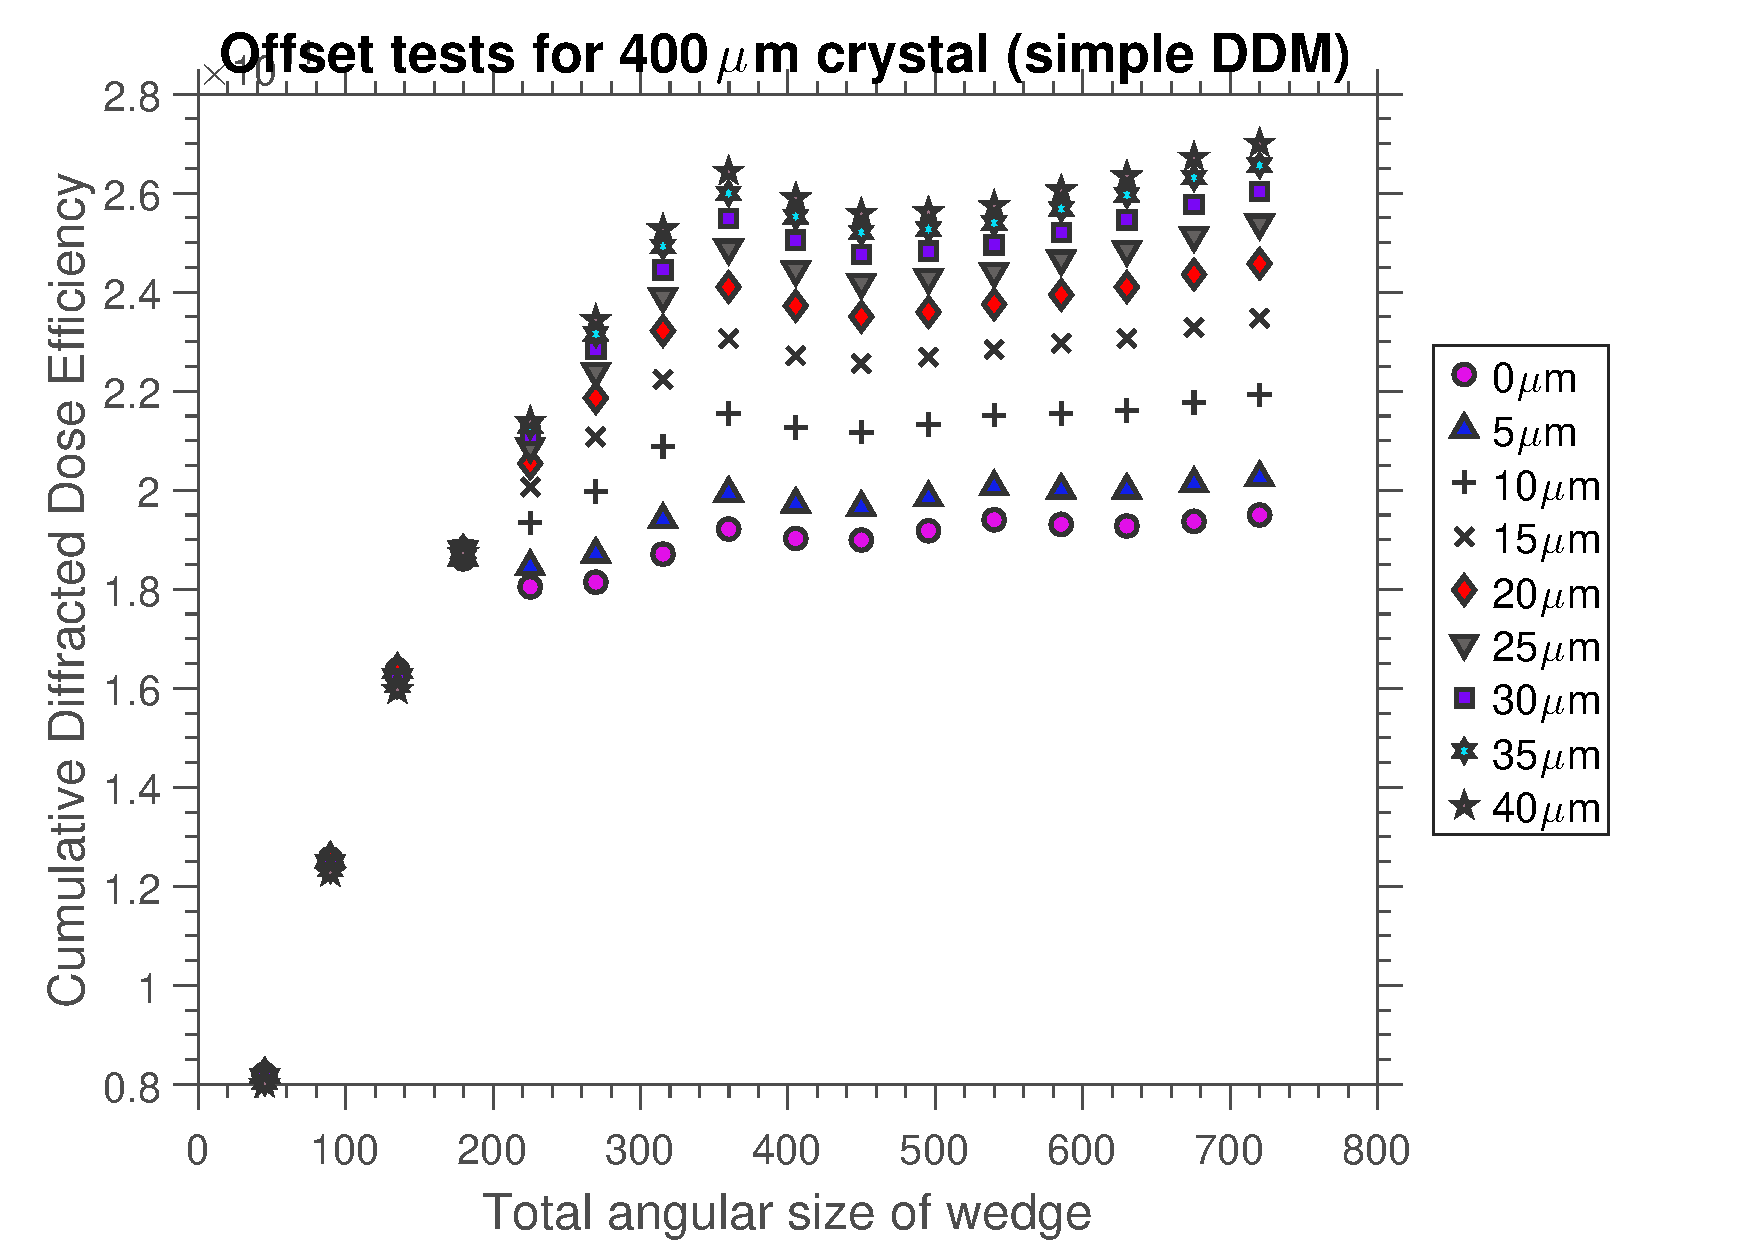
\includegraphics[width=\textwidth]{figures/dwd/OffsetSimulationDDMsimpleCrystSize400.pdf}
        \caption{}
        \label{fig:Offset simulations 400 - Simple Eta}
    \end{subfigure}
    \\
	\begin{subfigure}[b]{0.9\textwidth}
        \centering
        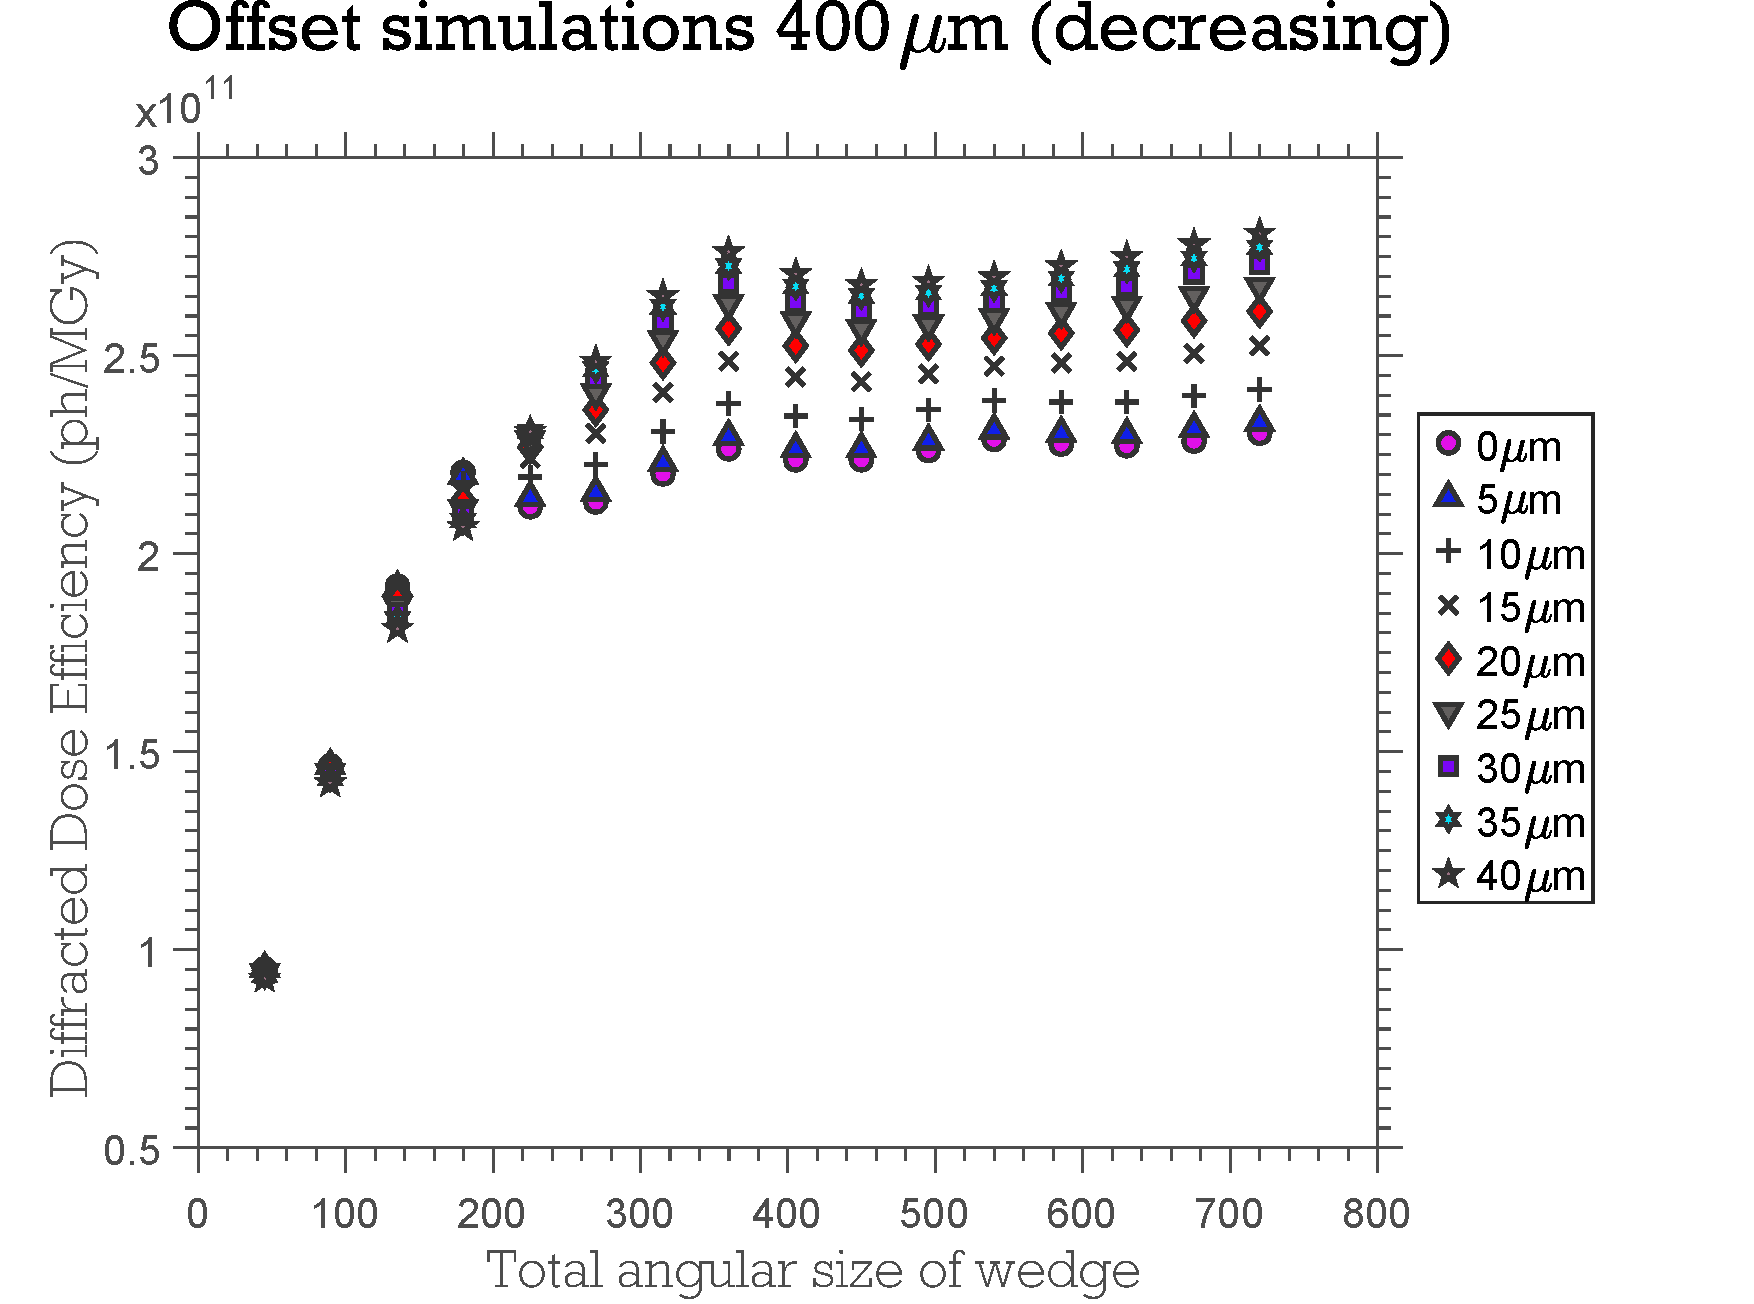
\includegraphics[width=\textwidth]{figures/dwd/OffsetSimulationDDMwrongCrystSize400.pdf}
        \caption{}
        \label{fig:Offset simulations 400 - Decreasing Eta}
    \end{subfigure}
\end{figure}
\begin{figure}
    \ContinuedFloat
    \begin{subfigure}[b]{0.9\textwidth}
        \centering
        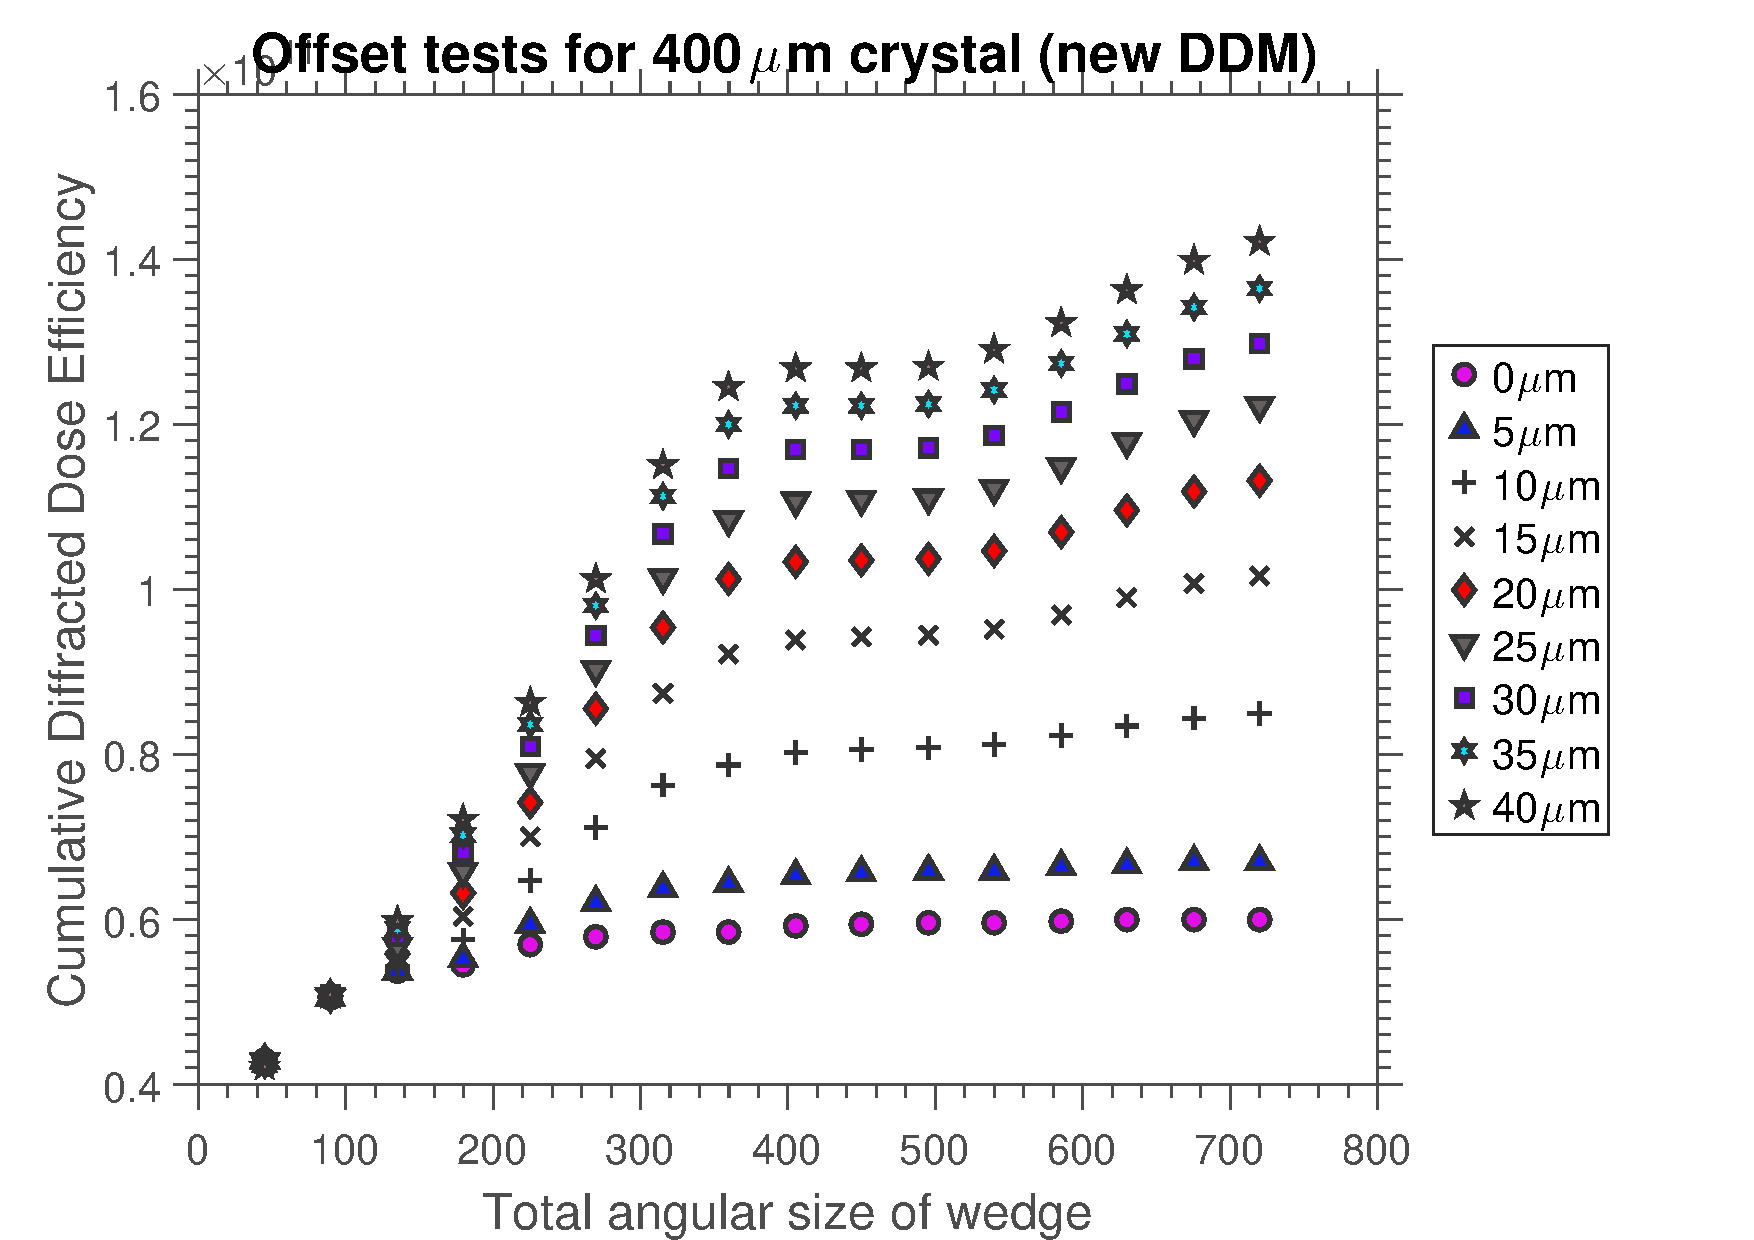
\includegraphics[width=\textwidth]{figures/dwd/OffsetSimulationDDMnewCrystSize400.pdf}
        \caption{}
        \label{fig:Offset simulations 400 - Increasing Eta}
    \end{subfigure}
    \\
    \begin{subfigure}[b]{0.9\textwidth}
        \centering
        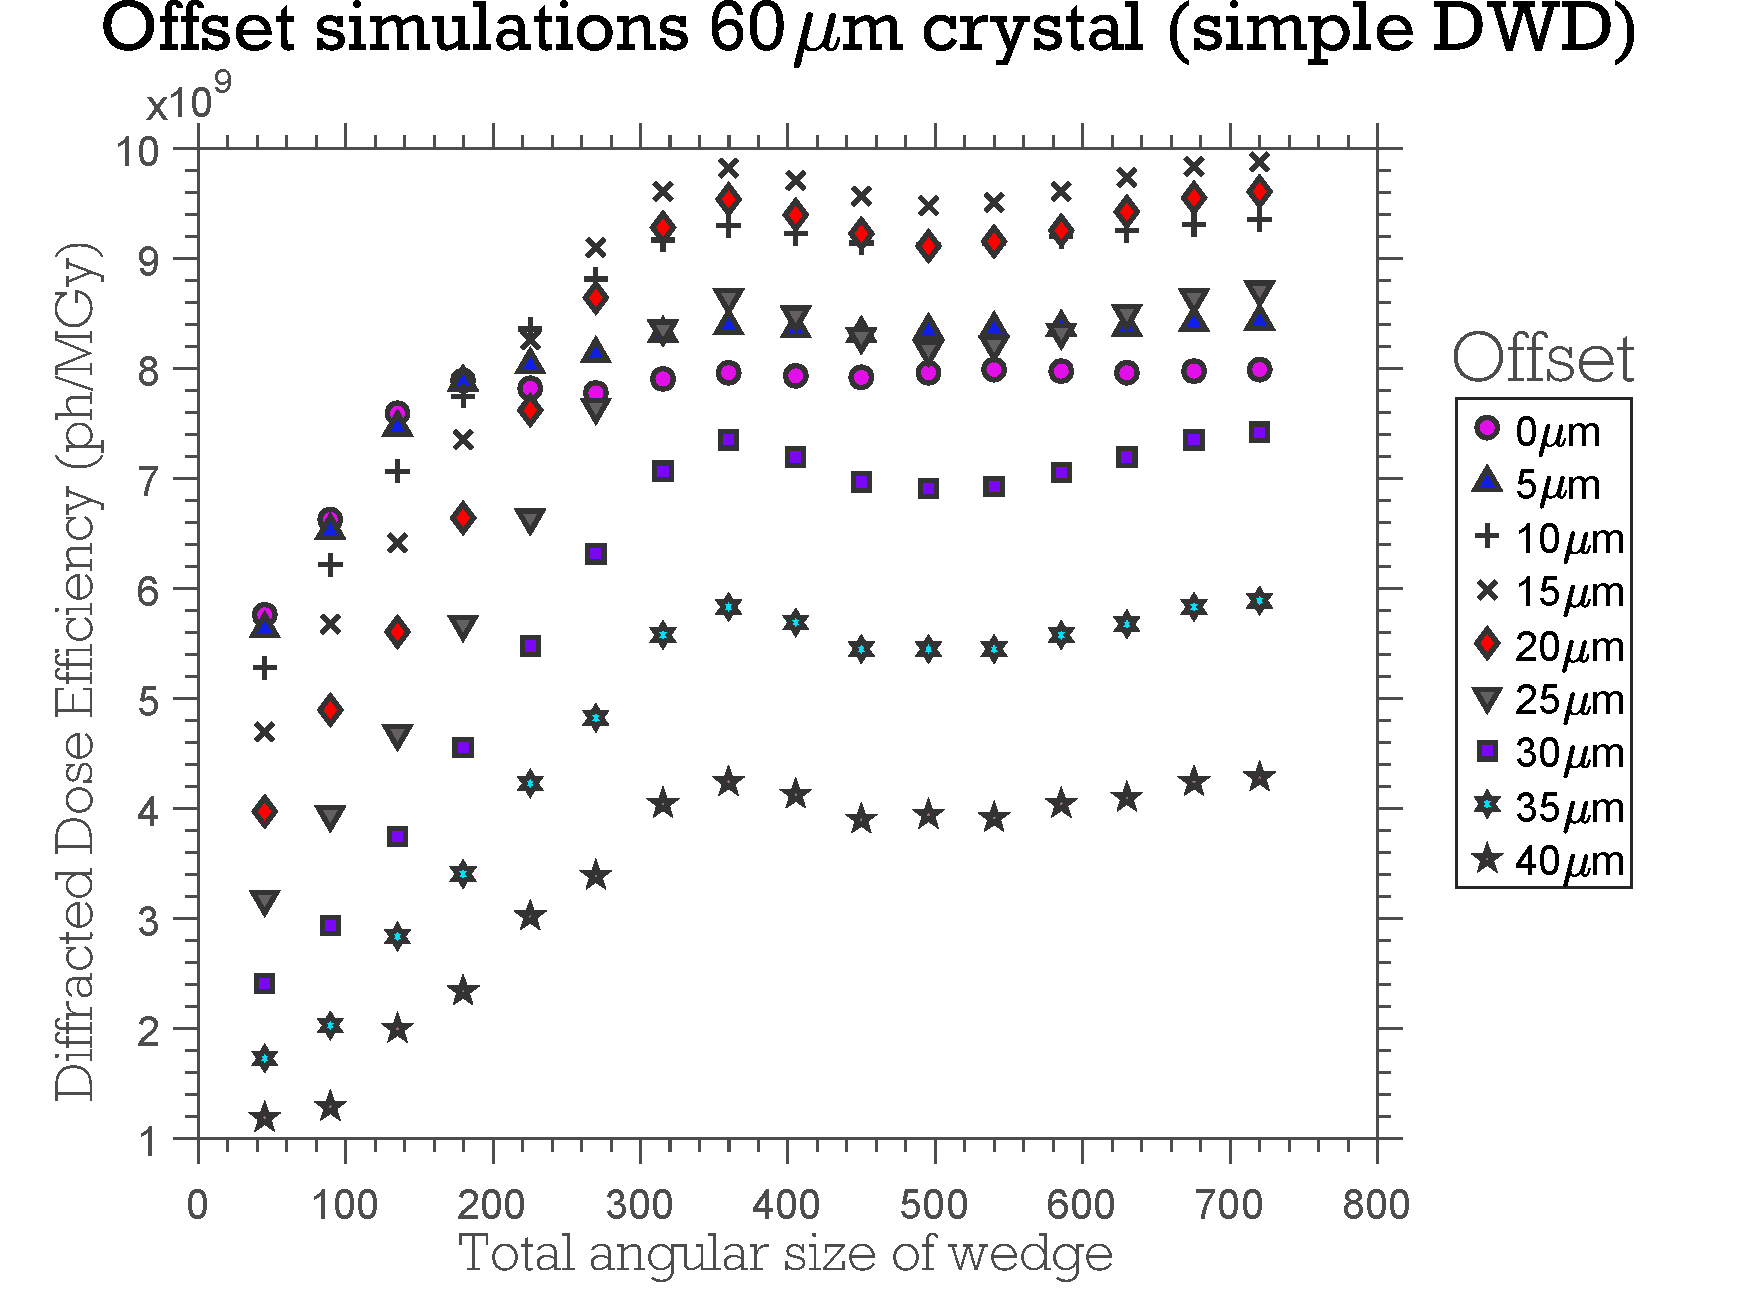
\includegraphics[width=\textwidth]{figures/dwd/OffsetSimulationDDMsimpleCrystSize60.pdf}
        \caption{}
        \label{fig:Offset simulations 60 - Simple Eta}
    \end{subfigure}
\end{figure}
\begin{figure}
    \ContinuedFloat
    \begin{subfigure}[b]{0.9\textwidth}
        \centering
        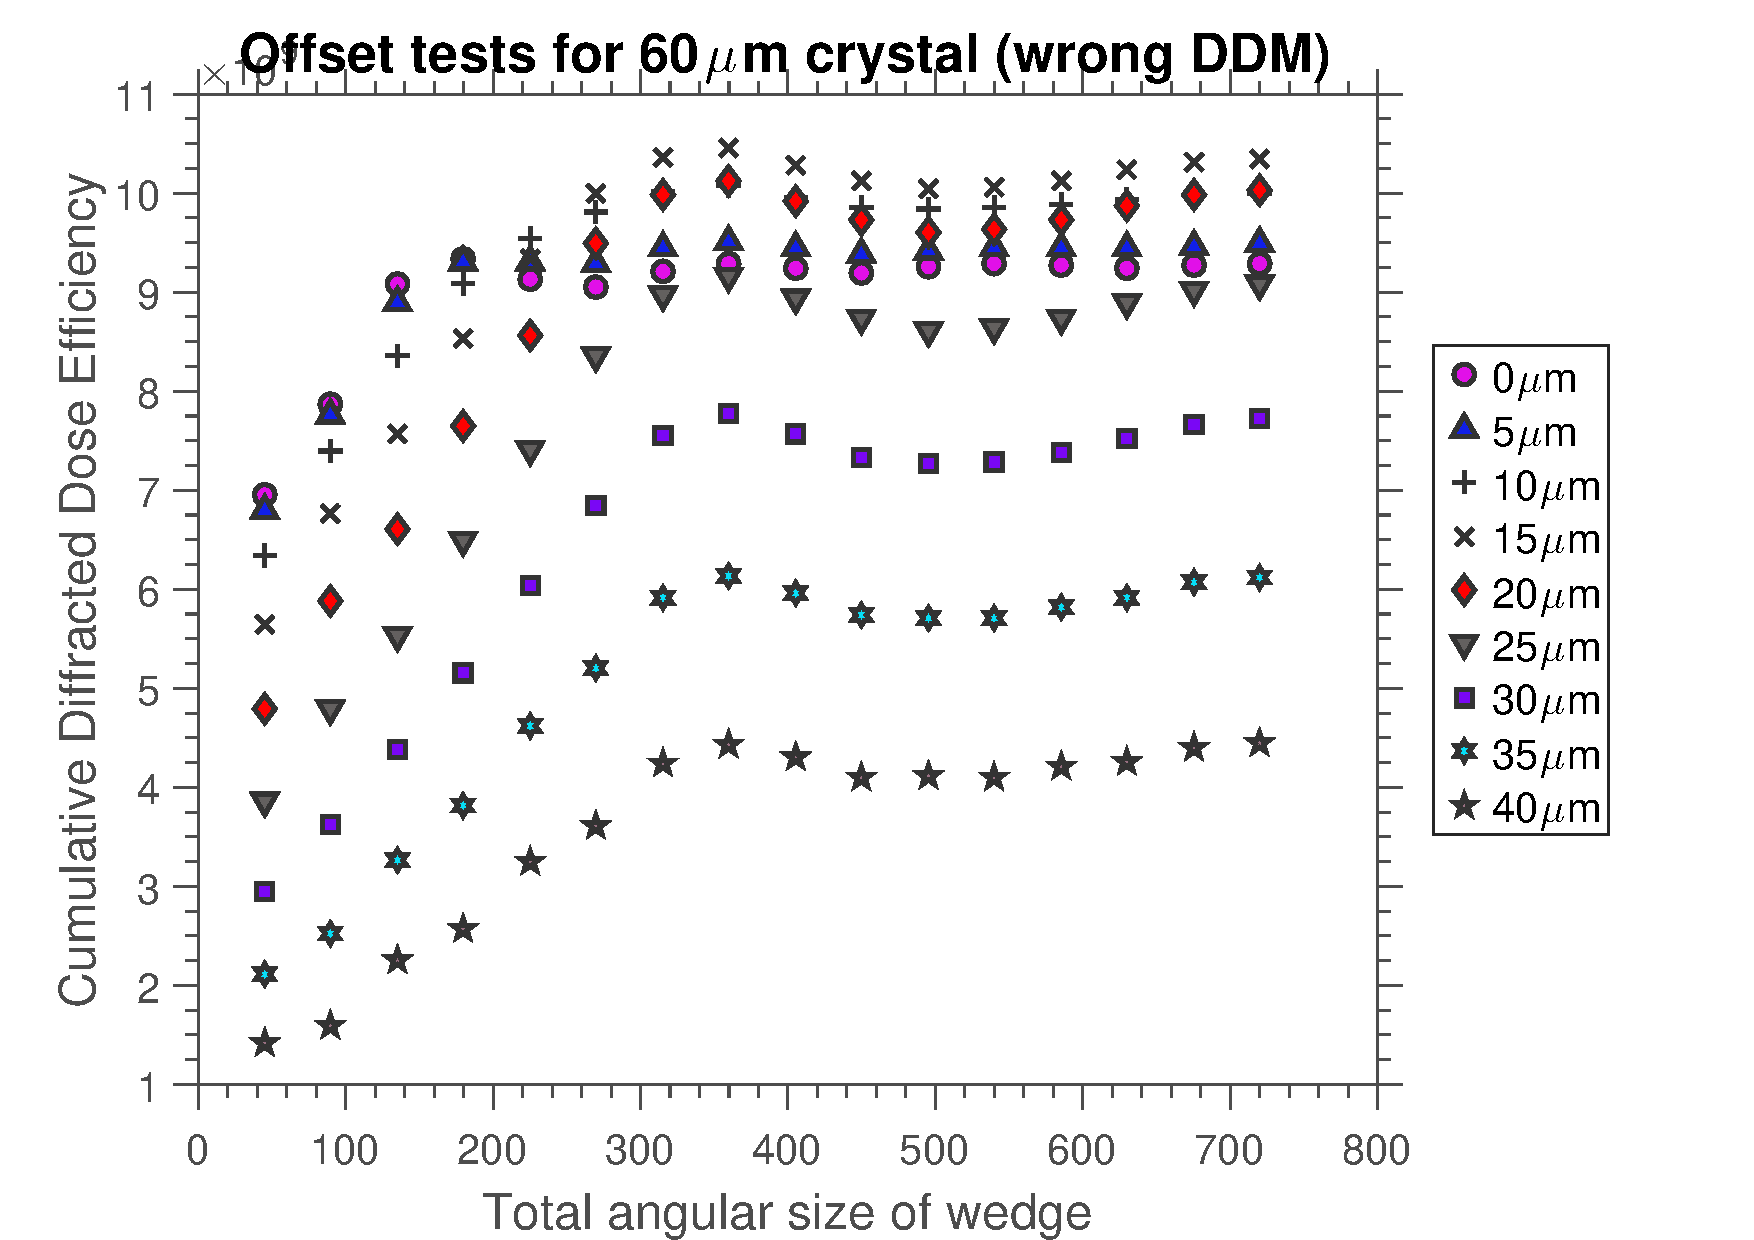
\includegraphics[width=\textwidth]{figures/dwd/OffsetSimulationDDMwrongCrystSize60.pdf}
        \caption{}
        \label{fig:Offset simulations 60 - Decreasing Eta}
    \end{subfigure}
    \\
    \begin{subfigure}[b]{0.9\textwidth}
        \centering
        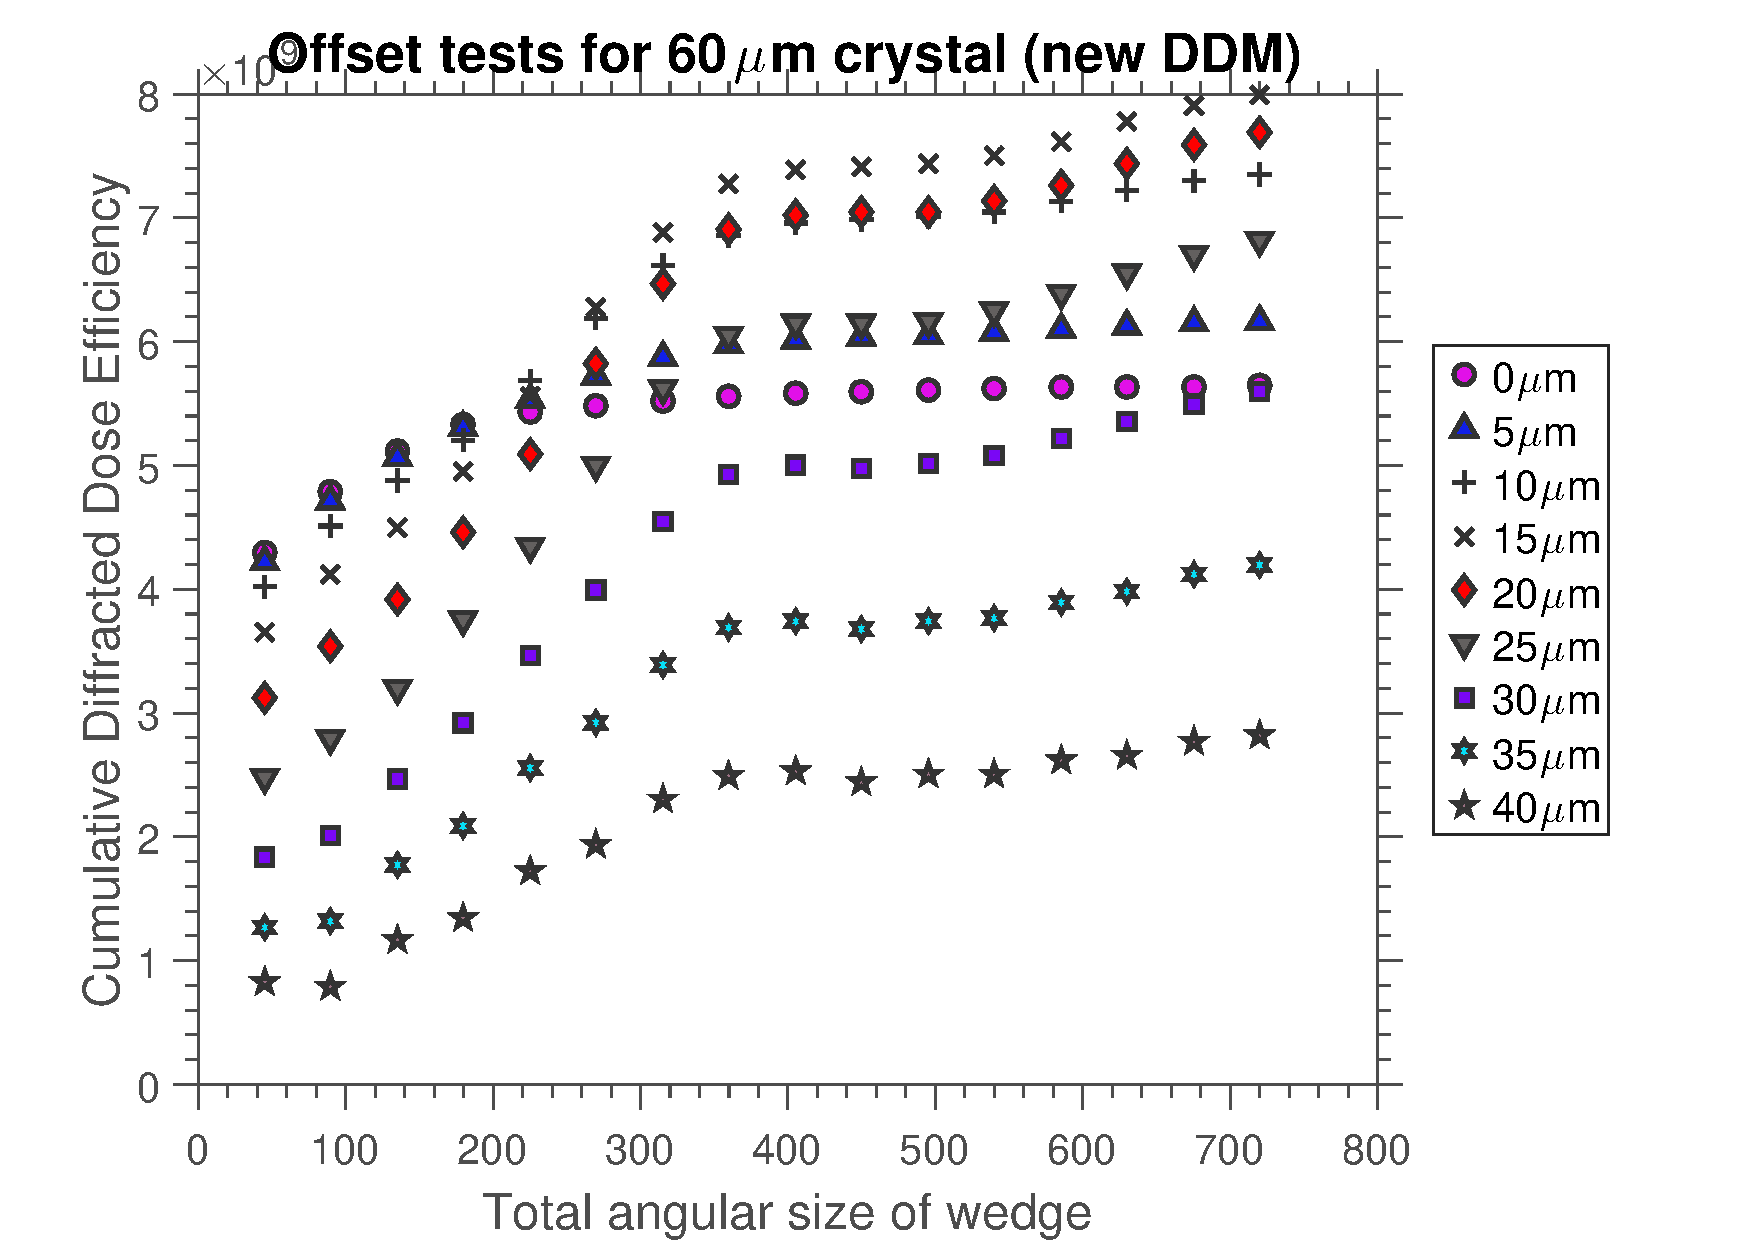
\includegraphics[width=\textwidth]{figures/dwd/OffsetSimulationDDMnewCrystSize60.pdf}
        \caption{}
        \label{fig:Offset simulations 60 - Increasing Eta}
    \end{subfigure}
    \caption{Results from the offset simulations showing the diffracted dose efficiency (DDE) plotted against the total rotation range for two different sized cubic crystals: 400$\,\mu m$ and 60$\,\mu m$ edge lengths.
    The DDE values are calculated from the DWD using the different forms of $\eta$ given by equations \ref{eq:Simple eta form}, \ref{eq:Decreasing eta form} and \ref{eq:Increasing eta form}}
    \label{fig:Offset simulations}
\end{figure}

\subsection{Offset Experiment}
\label{sub:Offset Experiment}
An experiment to validate the offset simulations was performed by Zeldin \textit{et al.} and reported in \cite{zeldin2013dwd}.
In the experiment a cuboid crystal of bovine pancreatic insulin (460 $\times$ 550 $\times$ 260$\,\mu m^3$) was irradiated in two regions with a beam of approximate size 40 $\times$ 70$\,\mu m^2$ (Figure~\ref{fig:Offset experiment - Beam}).
\begin{figure}
  \centering
    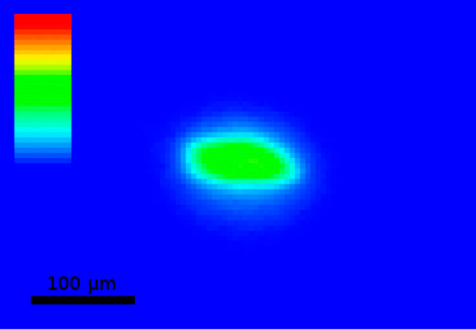
\includegraphics[width=0.75\textwidth]{figures/dwd/Oli_offset_exp_beam.png}
    \caption{False color images of the beam profile used in the offset experiment \cite{zeldin2013dwd}. The colorbar represents 0-255 intensity units.}
    \label{fig:Offset experiment - Beam}
\end{figure}
The first position corresponds to the rotation axis aligned with the beam axis (standard strategy).
The second position corresponds to the rotation axis offset from the beam axis by 1.25 times the beam FWHM (50$\,\mu m$ - offset strategy).
At each of the two positions three datasets were collected: first a 180$^{\circ}$ low dose \textit{probe} dataset, then a high-dose burn dataset, and then finally another low dose \textit{probe} dataset to evaluate the damage state of the crystal after it had been subjected to the high dose datasets.
To achieve the same DWD value (for the simple $\eta$ = 1 form) for each of the high dose datasets, the standard strategy exposed the crystal for 126 seconds whereas for the offset strategy the exposure was 162 seconds.
The final dose state of the crystal as calculated in RADDOSE-3D is shown in Figure~\ref{fig:Offset experiment - Dose state}.
\begin{figure}
  \centering
    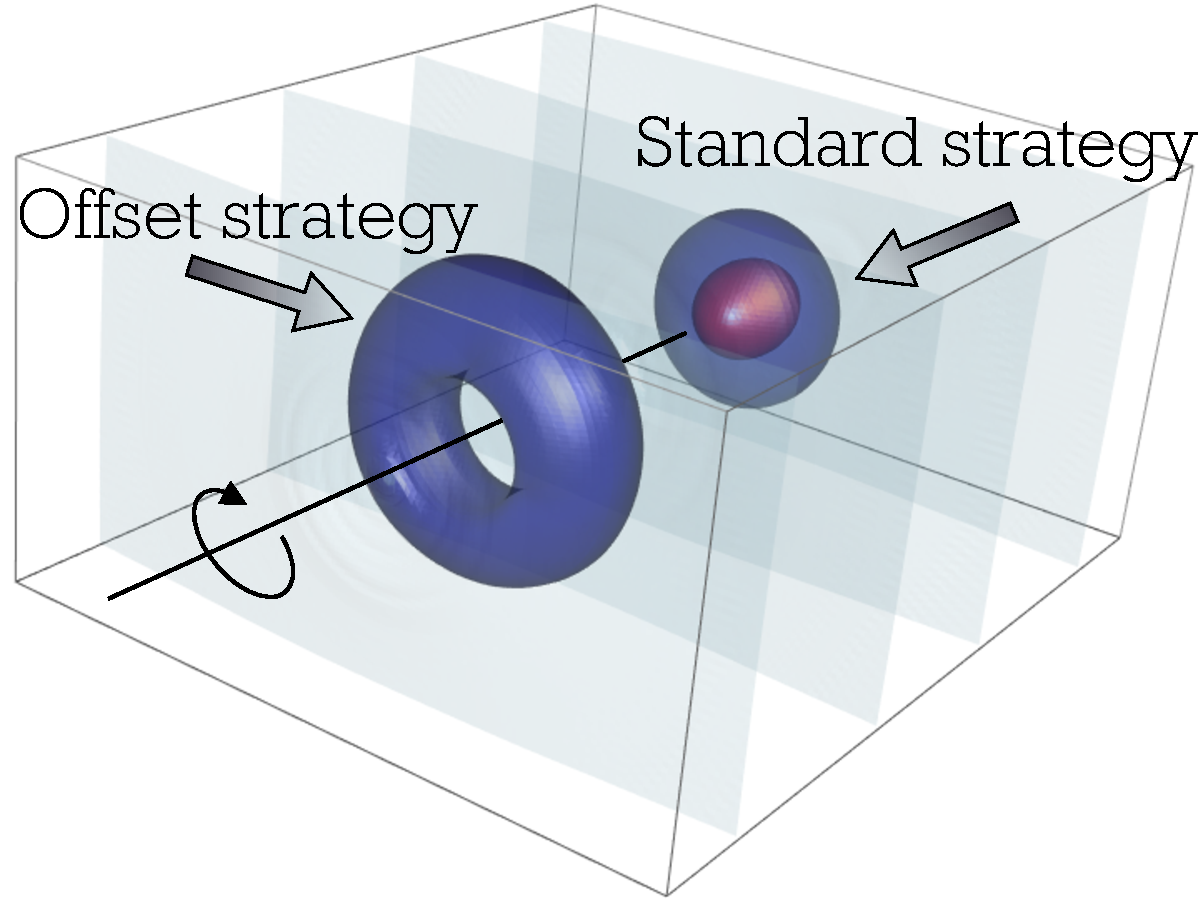
\includegraphics[width=0.8\textwidth]{figures/dwd/OffsetExperimentDoseState.pdf}
    \caption{Dose isosurface map for the crystal used in the offset experiment. Isosurfaces are at 0.1 MGy (light blue), 5 MGy (dark blue) and 10 MGy (red). Note that the dose at any point in the crystal for the offset experiment is lower than the maximum dose for the standard strategy.}
    \label{fig:Offset experiment - Dose state}
\end{figure}
The results from the data processing of this experiment with the different forms of DWD can be seen in Table~\ref{tab:Offset Experiment Results}.
\begin{table}[ht!]
\small
\captionsetup{justification=centering}
	\caption{The rows are presented in chronological order of the experiment. Syntax of the first column is: P1: 1st probe dataset, P2: 2nd probe dataset, HD: high dose dataset, -S: standard strategy, -O: offset strategy.}
	\centering
	\begin{tabular}{p{1.2cm} p{1.5cm} p{2cm} p{1.6cm} p{1.6cm} p{1.6cm}}
		Wedge   &Total time\footnotemark (s) &Elastic yield (ph)  &DWD simple $\eta$ (MGy)    & DWD decreasing $\eta$ (MGy)  &DWD increasing $\eta$ (MGy) \\
		\hline
		P1-S    & 5.4    & 5.5 $\times$ 10$^{\text{10}}$    & 0.08    & 0.08    & 0.16       \\
		P1-O    & 5.4    & 5.3 $\times$ 10$^{\text{10}}$    & 0.08    & 0.08    & 0.14       \\
		HD-O    & 162.0  & 1.6 $\times$ 10$^{\text{12}}$    & 1.86    & 1.77    & 2.85       \\
        HD-S    & 126.0  & 1.3 $\times$ 10$^{\text{12}}$    & 2.00    & 1.80    & 3.73       \\
        P2-S    & 5.4    & 5.5 $\times$ 10$^{\text{10}}$    & 3.81    & 1.77    & 7.03       \\
        P2-O    & 5.4    & 5.3 $\times$ 10$^{\text{10}}$    & 3.56    & 3.34    & 4.83       \\
		\hline
	\end{tabular}
	\label{tab:Offset Experiment Results}
\end{table}
\footnotetext{Equivalent at 100\% transmission (1.4 $\times$ 10$^{\text{12}}$ ph/s)}
The resulting DWD values for this experiment tell very different stories about the states of the crystal.
For the first probe datasets (P1-S and P1-O), the DWD using the decreasing $\eta$ agrees perfectly with those from of the DWD using the simple $\eta$ form.
The DWD values for the increasing $\eta$ form are practically double that value.
For the high dose datasets (HD-S and HD-O) that were designed so that the simple $\eta$ form DWD was similar for both strategies, the decreasing $\eta$ form DWD values for the two experiments are the most similar.
On the other hand, the increasing form $\eta$ DWD values differ by almost 1 MGy.
This result suggests either that the increasing $\eta$ form may not actually be representative of the real DWD (i.e. this is the incorrect form), or that the estimated DWD values with the other $\eta$ forms are misleading.
Finally there are several differences in the results for the second probe datasets (P2-S and P2-O).
The simple and increasing $\eta$ form DWD values suggest that the standard strategy results in a higher DWD value than the offset experiment.
This is the expected result.
The main difference however, is the large range in DWD values for the increasing $\eta$ DWD (2.2 MGy) compared to the range for the simple $\eta$ DWD (0.25).
Given that the relative intensity ($I_{n}/I_{1}$) for the standard and offset strategies for the second probe datasets are 0.79 and 0.85 respectively, the higher DWD difference could account for the relative intensity difference.
The DWD values using the decreasing $\eta$ form for the second probe datasets can be considered counterintuitive at first sight.
The result states that the DWD for the standard strategy is lower than the DWD for the high dose dataset which was taken before the second probe dataset.
If radiation damage is considered progressive then this result rules out using the decreasing form of $\eta$.
However it may be that the diffraction quality is better for the probe dataset than the high dose dataset, in which case this form of $\eta$ does not represent the level of damage, but instead, it is a dose value that describes the quality of the diffraction.
This result suggest that the relationship between the relative intensity and the DWD using the decreasing $\eta$ form is not a one-to-one function.
There are many possible relative intensity values for a given DWD value because the DWD can increase and then decrease again.
The DWD values are similar for the simple and decreasing $\eta$ forms for the offset strategy in the second probe experiment.
This is due to the fact that the dose for the offset experiment is smaller and hence the reduction of $\eta$ for the decreasing form was not significant enough to lower the DWD, as occurred for the standard experiment.
